%%%%%%%%%%%%%%%%%%%%%%%%%%%%%%%%%%%%%%%%%%%%%%%%%%%%%%%%%%%%%%%%%%%%
%% I, the copyright holder of this work, release this work into the
%% public domain. This applies worldwide. In some countries this may
%% not be legally possible; if so: I grant anyone the right to use
%% this work for any purpose, without any conditions, unless such
%% conditions are required by law.
%%%%%%%%%%%%%%%%%%%%%%%%%%%%%%%%%%%%%%%%%%%%%%%%%%%%%%%%%%%%%%%%%%%%

\documentclass[
  printed, %% This option enables the default options for the
           %% digital version of a document. Replace with `printed`
           %% to enable the default options for the printed version
           %% of a document.
  table,   %% Causes the coloring of tables. Replace with `notable`
           %% to restore plain tables.
  nolof,     %% Prints the List of Figures. Replace with `nolof` to
           %% hide the List of Figures.
  nolot,     %% Prints the List of Tables. Replace with `nolot` to
           %% hide the List of Tables.
           oneside, color
  %% More options are listed in the user guide at
  %% <http://mirrors.ctan.org/macros/latex/contrib/fithesis/guide/mu/fi.pdf>.
]{fithesis3}
%% The following section sets up the locales used in the thesis.
\usepackage[resetfonts]{cmap} %% We need to load the T2A font encoding
\usepackage[T1,T2A]{fontenc}  %% to use the Cyrillic fonts with Russian texts.
\usepackage[
  main=english, %% By using `czech` or `slovak` as the main locale
                %% instead of `english`, you can typeset the thesis
                %% in either Czech or Slovak, respectively.
  german, russian, czech, slovak %% The additional keys allow
]{babel}        %% foreign texts to be typeset as follows:
%%
%%   \begin{otherlanguage}{german}  ... \end{otherlanguage}
%%   \begin{otherlanguage}{russian} ... \end{otherlanguage}
%%   \begin{otherlanguage}{czech}   ... \end{otherlanguage}
%%   \begin{otherlanguage}{slovak}  ... \end{otherlanguage}
%%
%% For non-Latin scripts, it may be necessary to load additional
%% fonts:
\usepackage{paratype}
\def\textrussian#1{{\usefont{T2A}{PTSerif-TLF}{m}{rm}#1}}
%%
%% The following section sets up the metadata of the thesis.
\thesissetup{
    date          = \the\year/\the\month/\the\day,
    university    = mu,
    faculty       = fi,
    type          = mgr,
    author        = Bc. Radim Lipovčan,
    gender        = m,
    advisor       = RNDr. Vlasta Šťavová,
    title         = {Monero usage and mining from usable security view},
    TeXtitle      = {Monero usage and mining from usable security view},
    keywords      = {Monero, usable security, cryptocurrency, mining, pool, blockchain},
    TeXkeywords   = {Monero, usable security, cryptocurrency, mining, pool, blockchain},
}
\thesislong{abstract}{
    This is the abstract of my thesis, which can

    span multiple paragraphs.
}
\thesislong{thanks}{
    This is the acknowledgement for my thesis, which can

    span multiple paragraphs.
}
%% The following section sets up the bibliography.
\usepackage{csquotes}
\usepackage[              %% When typesetting the bibliography, the
  backend=biber,          %% `numeric` style will be used for the
  style=numeric,          %% entries and the `numeric-comp` style
  citestyle=numeric-comp, %% for the references to the entries. The
  sorting=none,           %% entries will be sorted in cite order.
  sortlocale=auto         %% For more unformation about the available
]{biblatex}               %% `style`s and `citestyles`, see:
%% <http://mirrors.ctan.org/macros/latex/contrib/biblatex/doc/biblatex.pdf>.
\addbibresource{Thesis.bib} %% The bibliograpic database within
                          %% the file `example.bib` will be used.
\usepackage{makeidx}      %% The `makeidx` package contains
\makeindex                %% helper commands for index typesetting.
%% These additional packages are used within the document:
\usepackage{paralist}
\usepackage{amsmath}
\usepackage{amsthm}
\usepackage{amsfonts}
\usepackage{url}
\usepackage{menukeys}

%packages
\usepackage{float} 
\usepackage{hyperref}
\usepackage[strings]{underscore}

%timeline
\usepackage{xcolor}
\newcommand\ytl[2]{
\parbox[b]{8em}{\hfill{\color{cyan}\bfseries\sffamily #1}~$\cdots\cdots$~}\makebox[0pt][c]{$\bullet$}\vrule\quad \parbox[c]{.7\linewidth}{\vspace{7pt}\color{red!40!black!80}\raggedright\sffamily #2.\\[7pt]}\\[-3pt]}

%caption
\usepackage{caption}

%branches
\usepackage{tikz}
%
\usetikzlibrary{trees}

%flowchart
\usetikzlibrary{shapes,arrows}
\usetikzlibrary{positioning}

%ringct
\usetikzlibrary{arrows,shapes,snakes,automata,backgrounds,petri}

%table
\usepackage{rotating}

%code
\renewcommand{\texttt}[1]{%
  \begingroup
  \ttfamily
  \begingroup\lccode`~=`/\lowercase{\endgroup\def~}{/\discretionary{}{}{}}%
  \begingroup\lccode`~=`[\lowercase{\endgroup\def~}{[\discretionary{}{}{}}%
  \begingroup\lccode`~=`.\lowercase{\endgroup\def~}{.\discretionary{}{}{}}%
  \catcode`/=\active\catcode`[=\active\catcode`.=\active
  \scantokens{#1\noexpand}%
  \endgroup
}

%images
\usepackage{graphicx}
\usepackage{float}
\graphicspath{ {./images/} }

%pdf
\usepackage{pdfpages}

%piechart
\usepackage{pgf-pie}

%multicol
\usepackage{multicol}

%code
\usepackage{listings}
\usepackage{color}

\definecolor{dkgreen}{rgb}{0,0.6,0}
\definecolor{gray}{rgb}{0.5,0.5,0.5}
\definecolor{mauve}{rgb}{0.58,0,0.82}

\lstset{frame=tb,
  language=Java,
  aboveskip=3mm,
  belowskip=3mm,
  showstringspaces=false,
  columns=flexible,
  basicstyle={\small\ttfamily},
  numbers=none,
  numberstyle=\tiny\color{black},
  keywordstyle=\color{black},
  commentstyle=\color{black},
  stringstyle=\color{black},
  breaklines=true,
  breakatwhitespace=true,
  tabsize=3
}
\begin{document}

\chapter{Introduction}
%% Komentář Vlasta 10.7.: tady někde (možná samostatná kapitola) bude nutné nadefinovat pojmy. Nazvat to "Kryptoměny" a popsat tam myšlenku, z čeho se skládají, co je blockchain, co to znamená fork... a tak.
%% Komentář Vlasta 10.7.: Nechceš to psát anglicky? Myslím, že by sis tím ušetřil hromadu práce s překlady. Dotazník bude v jakém jazyce?

%% Komentář Radim 13.07: Kapitola s pojmy - udělám zvlášť krátkou, ve které popíšu tyto základní principy, ještě tedy před Monero Cryptocurrency kapitolou. Monero specific věci pak budou popsány už pod Monerem.
%% Komentář Radim 13.07: Po domluvě mailem tedy začnu psát Anglicky. Dotazníky budou ve dvou jazykových mutacích - ENG a CZ. Hlavně kvůli CZ komunitě těžařů a pool operátorům - https://bohemianpool.com/#/home bych dal i tu češtinu.
\chapter{Cryptocurrency}
\textbf{Cryptocurrency} is a digital currency that is designed to use cryptography to secure and verify its transactions. Cryptocurrencies are decentralized as opposed to traditional money transaction systems used in the banks. Decentralisation is established by using distributed blockchain that functions as a transaction database within the currency. First cryptocurrency available was Bitcoin \cite{farell2015analysis}.

\textbf{Altcoin} is a term used for every cryptocurrency that is not Bitcoin as it is a direct concurrent for the first of the cryptocurrency.

The \textbf{fork} happens when developers create a copy of existing project codebase and start their individual path of development with it. 

\textbf{Market Cap} is a total value of cryptocurrency that refers to the total number of emitted coins multiplied by the value of the coin.

\textbf{The blockchain} is a technology responsible for storing every transaction that has ever been processed in the cryptocurrency, also often called as a ledger. The main purpose of the blockchain is to ensure the validity of completed transactions.

\textbf{Transactions} within cryptocurrency are processed together as blocks that are verified by miners and then added to the blockchain as a new mined block.

\textbf{The wallet} is a storage medium that holds private and public keys by which user can access, send and receive funds. Wallet effectively does not have the coins but is rather a key to access them from the blockchain.

\textbf{Node} is a computer connected to the cryptocurrency network. Node is often referred to as a full node which means that the computer maintains a full copy of blockchain. This results in node downloading every block and transaction and checking them against cryptocurrency rules, especially whether the transaction has correct signatures, data format and the right number of emitted coins per block.

\textbf{Mining} process is done by miners that verifies transactions on the network and adds them to the blockchain together in form of a block which results in new coins being emitted as a reward for block solving.

\textbf{Mining in pools} is the way how individual miners pool their computational resources. Due to resources pooling, there is a higher chance of solving the block thus gaining the reward of newly emitted coins. %After solving each block, the reward is distributed equally to miners connected to the pool according to PPS or PPLNS system.

\chapter{Monero Cryptocurrency}
Monero is an open-source cryptocurrency that is developed under the Monero project in order to create a decentralized and anonymous currency. Its main goal is to make the user the one who has complete control over own funds.

Meaning that every single digital transaction and the exact number of coins in users wallet cannot be traced back to the user without sharing the view key of the transaction \cite{moneroprojectgithub}. Main distinctive points compared to other cryptocurrencies are:

\begin{itemize}\itemsep0em
\item The blockchain is public, but a large part of it is encrypted.
\item The sender of the transaction is hidden by using Ring Signatures explained in chapter  \ref{sec:ringsignatures}.
\item The exact amount of transferred coins is encrypted using RingCT as described in \ref{sec:ringct}.
\item Transaction history and receiving party is hidden by the usage of stealth addresses that are referenced in chapter \ref{sec:stealthaddresses}.
\end{itemize}

\section{Origin and the main focus}
Monero started its way by forking from Bytecoin, which was proof-of-concept cryptocurrency that used as first of its kind protocol called CryptoNote. CryptoNote was published by the start of the year 2014 \cite{githubbytecoin}.

Although Bytecoin had a promising protocol aimed at privacy, there was a problem with premine, meaning that cryptocurrency at the time of publishing had already 82\% of the coins already emitted \cite{fluffyponyonbytecoin}. That was the reason why people interested in anonymous cryptocurrencies decided to create a Bytecoin fork under the name of BitMonero \cite{bitmonero}. 

Next important moment was when a significant part of the developers decided to abandon the project in favor of creating a new fork named Monero in 06.23.2014. By this action, Monero cryptocurrency was created with publicly known blockchain from the start, strictly defined goals and motivated team of developers \cite{monerofork}.

%% Komentář Vlasta 10.7.: Návrh: v téhle kapitole by bylo moc hezká nějaká přehledová tabulka cca 5 největších kryptoměn, kde bys je porovnal podle vybraných kriterii. Třeba kriterium "Množství odesílané měny je šifrováno" by bylo v sloupečku a v pro každou kryptoměnu na řádek vyznačil, zda to splňuje nebo ne. Bylo by pak přehledně vidět čím je Monero tak vyjimečné a jak jsou na tom v těhle kriteriích ostatní kryptoměny.

%% Komentář Radim 4.8.: Tabulku jsem udělal, akorát ještě musím zakomponovat sloupec, který ukazuje samotný market cap. Spíš jsem se totiž nejdříve zaměřil, jak top5 crypto vypadá z hlediska privacy features. Tzn. dávám si tu DOPLNIT .

\section{Monero market cap}
 As Monero is often mentioned for its privacy features, decentralization in mind and fungibility as main asset, table \ref{table:monero-top5} puts Monero in the direct comparison against top 5 cryptocurrencies.

To compare different cryptocurrency projects, market capitalization (market cap) is often used as a way of ranking \cite{elbahrawy2017evolutionary}. It indicates the relative size of cryptocurrency by the formula: \\ \centerline{
 \textit{\textit{Market Cap = Circulating Supply * Price} }}
 
\textbf{Privacy} in cryptocurrency is a feature that assures that amount of coin user owns, sends or receives cannot be seen on the blockchain.

\textbf{Decentralization} in cryptocurrency network all nodes are equals. That means that no supernode can override how transactions are being processed as well as there is no single entity in control.

\textbf{Fungibility} means that every coin ever emitted has the same value as the others and cannot be traced back thus there cannot be coin blacklist.

\begin{figure}[H]
\centering\begin{tabular}{{p{0.06\linewidth}p{0.13\linewidth}p{0.17\linewidth}p{0.15\linewidth}p{0.15\linewidth}p{0.15\linewidth}}}
\textbf{Rank} & \textbf{Name} & \textbf{Transactions per day} & \textbf{Privacy}               & \textbf{Decentra-lization} & \textbf{Fungibility}            \\
1    & Bitcoin        & 225039          & No & Yes              & No  \\
2    & Ethereum       & 610953          & No &   Yes               & No                       \\
3    & XRP            & 633974          & No                      &     No	             &                       Varies \\
4    & Bitcoin Cash   & 125404          & No &        Yes          &          No              \\
5    & EOS            & 406380          &      No                 &                 Yes &                 Varies       \\
13   & Monero         & 4010             &     Yes                  &                 Yes &      Yes                                                                                      
\end{tabular}
\captionof{table}{Monero features in top 5 cryptocurrencies.}
\label{table:monero-top5}
\end{figure}
As can be seen from data in table \ref{table:monero-top5}, coins that are most popular by market cap metrics, are not centered around privacy. Altought it is often believed that using cryptography means anonymity, it isn't true in most cryptocurrencies especially in Bitcoin \cite{conti2018survey}. 

XRP and EOS are in a unique position compared to typical cryptocurrency as they offer a crypto platform with contracts, so privacy implementation and fungibility varies from contract to contract \cite{domingues2018allvor}.
%Zdroj transaction volume: https://bitinfocharts.com/monero/
%Zdroj Bitcoin: https://bitcoin.org/en/protect-your-privacy
%Zdroj Ethereum: https://ieeexplore.ieee.org/document/8356459/
%Zdroj XRP: https://ieeexplore.ieee.org/document/8356459/
%https://ripple.com/insights/xrp-compares-btc-eth/
%https://bitcoinist.com/not-decentralized-ripple-freezes-1m-user-funds/
\newpage
\section{Monero competitors}
\label{sec:monero-timeline}
Monero is not the only one cryptocurrency that aims at privacy and anonymity features, and there are many privacy coins already in existence. Most similar to Monero is ByteCoin from which Monero was forked, but is overall unpopular due to 82\% premine.  A viable alternative to Monero offers its fork Aeon that is more lightweight as opposed to Monero with slightly fewer privacy features.

\begin{figure}[H]
\centering
\begin{tabular}{p{0.1\linewidth}p{0.16\linewidth}p{0.1\linewidth}p{0.15\linewidth}p{0.15\linewidth}p{0.15\linewidth}}
\textbf{Name}        & \textbf{Protocol}                & \textbf{Block Time {[}s{]}} & \textbf{Stealth Address    }      & \textbf{Anonymous transactions} & \textbf{Transaction signing}  \\
Aeon         & CryptoNote-Light        & 240                & Yes                      & Yes                & Ring Signature \\
Byte-Coin     & CryptoNote              & 120                & Yes                      & Yes                & Ring Signature \\
DASH         & X11                     & 150                & No                       & Not fully           & Yes            \\
Monero (XMR) & CryptoNote              & 120                & Yes                      & Yes                & RingCT         \\
PIVX         & Zerocoin                & 60                 & Partialy & Yes                & x              \\
Verge (XVG)  & Scrypt                  & 150                & Yes                      & Ne, TOR\&I2P       & RingCT WIP     \\
Zcash (ZEC)  & Zerocash                & 150                & Shielded addresses  & Yes by SNARKS    & x              \\
Zcoin (XZC)  & Lyra2 =\textgreater MTP & 600                & Yes                      & Yes by minting \& spending  & Ring Signature

\end{tabular}
\captionof{table}{Comparison of Anonymous Cryptocurrencies and their features.}
\label{table:monero-alternatives}

%Zdroje:
%dash https://bitcointalk.org/index.php?topic=1562109.0
%ďash https://docs.dash.org/en/latest/introduction/information.html
%pivx https://github.com/PIVX-Project/PIVX
%pivx https://www.reddit.com/r/pivx/comments/7gjjyw/what_are_the_benefits_of_multisig_addresses/
%zcoin https://github.com/zcoinofficial/zcoin/wiki/Information-for-exchanges
%zcoin https://zcoin.io/zcoins-privacy-technology-compares-competition/

\end{figure}
Information sources used in table \ref{table:monero-alternatives} and in the picture \ref{pict:monero-alternatives-codebase}:\\
Aeon \cite{moneroalternativeaeon}, ByteCoin \cite{moneroalternativebytecoin}, Dash \cite{moneroalternativedash,moneroalternativedashdev}, Monero \cite{moneroprojectgithub}, Pivx \cite{moneroalternativepivx}, Verge \cite{moneroalternativeverge}, Zcash \cite{moneroalternativezcash}, Zcoin \cite{moneroalternativezcoin}.
\iffalse
\begin{figure}[H]
\centering
\begin{tikzpicture}[sibling distance=10em,
  every node/.style = {shape=rectangle, rounded corners,
    draw, align=center,
    top color=white, bottom color=blue!20}]]
  \node {Bytecoin}
	child { node {DASH} 
	child { node {PIVX}}}
    child { node {BitMonero}
      child { node {Monero}
        child { node {AEON} } } };
      \node[xshift=21mm]{Verge};
        \node[xshift=4cm] {Bitcoin}
	child[xshift=25mm] { node {Zcash}}
	child[xshift=0cm] { node {Zcoin}};  
\end{tikzpicture}
\caption{Codebase overview of the selected cryptocurrencies.}
\label{pict:monero-alternatives-codebase}
\end{figure}
\fi
%verge ma svoji codebase "non-bitcoin coin" viz prvni commit https://github.com/PIVX-Project/PIVX/commit/4405b78d6059e536c36974088a8ed4d9f0f29898

\section{Development cycle}
%% Komentář Vlasta 10.7.: Trochu popiš jak moc je Monero rozšířené. Pro představu v porovnání s dalšími kryptoměnami. Aby bylo jasné, že to není nějaká obskurní kryptoměna.

Monero development cycle is based on planned network updates that occur every six months. By this developers want to encourage work on the project with regular updates in contrast to other cryptocurrencies that don't want any new hard forks in the future as it brings the danger of splitting the coin into several versions \cite{mccorry2017atomically}.

\begin{figure}[H]
\center
\color{gray}
\rule{\linewidth}{1pt}
\ytl{03.03.2014}{Bytecoin - published on GitHub}
\ytl{04.17.2014}{ByteCoin fork - the creation of BitMonero cryptocurrency}
\ytl{07.23.2014}{BitMonero Fork - the creation of Monero cryptocurrency}
\ytl{03.22.2016}{Monero v2 - ring size change, block time set to 120 seconds}
\ytl{09.21.2016}{Monero v3 - transactions are split into smaller amounts}
\ytl{01.05.2017}{Monero v4 - the concurrent run of normal and RingCT transactions}
\ytl{04.15.2017}{Monero v5 - block size update and fee algorithm adjustments}
\ytl{09.16.2017}{Monero v6 - RingCT forced on the network with ring size => 5}
\ytl{04.06.2018}{Monero v7 - change of CryptoNight mining algorithm to prevent ASIC on the network, ring size set to =>7}
\ytl{10.--.2018}{Future network update}
\bigskip
\rule{\linewidth}{1pt}%
\color{black}\caption{Monero development timeline.}
\label{monero-timeline}
\end{figure} \newpage

Updates are meant to improve and enhance the previously established codebase as well as fixing already existing bugs that are continuously being resolved. Known problems in Monero history were:

\begin{itemize}
\item \textbf{Spam attack}
\begin{itemize}
\item Was aimed to oversaturate the Moneros network by sending minimal transactions and leveraging low transaction fee of 0.005 XMR. Immediate fix was established by raising the fee to 0.1 XMR. This problem led to the implementation of dynamic transaction fee based on chosen transaction priority \cite{monerospamattack}.
%zdroj https://bitcointalk.org/index.php?topic=583449.msg8519146#msg8519146
\end{itemize}
\item \textbf{Split chain attack}
\begin{itemize}
\item The successful exploit of Merkle root calculation vulnerability led to the creation of two blocks of the same height and hash, but with two different transactions on the end of the block \cite{macheta2014counterfeiting}. By this, two separate Monero chains were created. Exploit applied to all CryptoNote based cryptocurrencies. In the case of Monero, all transactions were stopped on exchanges until next day, when the fix was issued \cite{cryptonotemerkletree}.
\end{itemize}
\item \textbf{Transaction analysis in Monero blockchain}
\begin{itemize}
\item Research published in 2017 uncovered past and present problems in anonymity with Monero transaction system. The most significant discovery was that a substantial portion of transactions used a ring signature of zero which caused traceability of the amount of coin in the transaction output on the blockchain \cite{moser2018empirical}.
\item This issue was resolved by Monero team already in 2016 with Monero v2, where ring signature was set to =>3 \cite{monerov2release}. Soon after the paper was released, Monero got its v6 update with enforced use of RingCT technology for all transaction outputs \cite{monerov6release}.
\end{itemize}
%zdroj https://eprint.iacr.org/2017/338.pdf
\end{itemize}
%zdroj https://getmonero.org/2017/05/17/disclosure-of-a-major-bug-in-cryptonote-based-currencies.html
\newpage
\section{Transactions in Monero network}
Monero uses a distributed peer-to-peer consensus network to record transaction outputs in a blockchain. That means that balance is not stored in a wallet, but is represented by control over outputs of transactions accessible with wallet keys \cite{seguias2018moneroa}.

By that when user A wants to send funds to user B, the transaction happens in the way of transformation of controlled outputs in one wallet to a new output that belongs to the other wallet. As this is only a principle how coins are transferred between wallets Monero uses additional technology to make transactions private.
\subsection{Monero wallet and stealth addresses}
\label{sec:stealthaddresses}
Monero wallet seed is 95 characters long string that consists of public view and spend key. To send funds from one wallet to another, a one-time public key is created, that contains senders public view and spend key as well as randomized data. 

This one-time public key is also referred to as a stealth address and is generated and recorded as part of the transaction to set the controller of the output of the transaction \cite{seguias2018monero}.

Stealth address is visible on the blockchain, by this receiving party can scan the blockchain to find exact transaction using their private view key. After locating transaction output, wallet software is then able to calculate one-time private key that aligns with one-time public key and can spend this output using private spend key \cite{courtois2017stealth}.

By this, no one from outside can link nor wallet addresses nor people involved in a particular transaction by scanning the blockchain as there is no association with receivers address.

To prove that funds were sent from one wallet to another, the sender has to disclose transactions ID, receivers address and transactions key.

\subsection{Ring Signatures}
\label{sec:ringsignatures}
Ring signatures present a way how to create a distinctive signature that authorizes a transaction. The digital signature of the transaction is compiled from the signer together with past outputs of transactions (decoys) to form a ring where all members are equal and valid. By that, outside party cannot identify exact singer as it is not clear which input was signed by one time spend key\cite{mercer2016privacy}.

To prevent double spend, a cryptographic key image is derived from the spent output and is part of the ring signature. As each key image is unique, miners can verify that there is no other transaction with the same key image, thus preventing the double-spending attack \cite{miller2017empirical}.

\subsection{RingCT}
\label{sec:ringct}
So far, senders anonymity is ensured by ring signatures, receivers anonymity relies on stealth addresses, but the amount of Monero transferred would be still visible on the blockchain. To hide transaction amounts, Ring Confidential Transactions are implemented \cite{noether2015ring}.

As one output cannot be spent twice, the sender has to spend entire output in the transaction. That typically results in a transaction having two outputs, one for the receiver and one for the original wallet, where the excess amount of coins is returned.	 

To prevent manipulation during a transaction, the total input amount must equal the output amount of coins in each transaction. As one could exploit this by committing to value less than zero, range proofs are there to ensure cryptographic evidence of amounts used in transactions is greater than zero and falls into the valid transaction amount range. 

To confirm the transaction, the sender reveals the masked amount of coins being sent in the transaction to the network that is later verified by miners \cite{sun2017ringct}. 

By that, amounts transferred between wallets in the form of outputs of transactions are hidden, and the network can still confirm that transaction is valid.

\subsection{Kovri}
Kovri is a C++ implementation of the I2P anonymous network under heavy development process in Monero project. It aims to offer secure network transmissions where a user's IP cannot be associated with a particular transaction ID \cite{monerokovri}. 

\chapter{Monero usage}
As pointed out in section \ref{sec:monero-timeline}, Monero is one of the cryptocurrencies that aim to implement as complex anonymity system as possible. Moreover, because of that not only the underlying technology of the network is different from other cryptocurrency projects but the user side as well. 
\section{Wallets}
\label{sec:wallets}
The essential part of every currency is the user's ability to access stored funds. In cryptocurrency, this is represented by the wallet and associated software.

Monero wallet contains information that is necessary to send and receive Monero currency. Each wallet is encrypted by the password set in the creation process. Typical wallet created using Monero software named \textit{example-wallet} consists of:
\begin{itemize}\itemsep0em
\item \textbf{example-wallet.keys file}
\begin{itemize}\itemsep0em
\item Is an encrypted file containing private \textbf{spend key} and \textbf{view key} together with \textbf{wallet address}.
\item Keys file also contains user preferences related to transactions and wallet creation height, so wallet software will only read blockchain from the wallet creation point.
\item Using this file, the user can restore wallet by using the monero-wallet-cli command: monero-wallet-cli --generate-from-keys
\end{itemize}
\item \textbf{example-wallet file}
\begin{itemize}\itemsep0em
\item Acts as an encrypted cache for wallet software that contains:
\begin{itemize}\itemsep0em
\item List of outputs of transactions that are associated with the wallet as it does not need to scan the blockchain every time after startup.
\item History of transactions with metadata containing tx keys.
\end{itemize}
\end{itemize}
\item \textbf{example-wallet.address.txt file}
\begin{itemize}\itemsep0em
\item Stores \textbf{unencrypted} information containing generated wallet address.
\item With recent address-based attacks that swap wallet addresses found in clipboard or files on the hard drive for the attacker's wallet address, this poses a security risk \cite{cryptoshuffler}.
\end{itemize}
\item \textbf{Mnemonic seed}
\begin{itemize}\itemsep0em
\item Mnemonic seed is a 25-word phrase which the last word is being used as a checksum. Together they represent a 256-bit integer that is the accounts private spend key.
\item By having accounts private spend key, wallet software can derive private view key by hashing private key with Keccak-256. That produces another 256-bit integer that represents private view key.
\item Both public keys are then derived from newly recovered private keys.
\end{itemize}
\end{itemize}
Example of Monero wallet address and mnemonic seed:
\begin{itemize}\itemsep0em
\item \textbf{Wallet address}
\begin{itemize}\itemsep0em
\item 461TWLQhsxrR9dD4CXk4p1RRxAAQ3YCEDhNiGCQjj5\\QA33ohhZPnCX6346EyEwC7TiRSB3XB8KgNaJ4vThd5N\\pQqRkGab66
\end{itemize}
\item \textbf{Mnemonic seed}
\begin{itemize}\itemsep0em
\item serving odometer nifty flippant worry sphere were thorn putty bogeys lyrics feast fawns input biscuit hobby outbreak rash tucks dwelt liquid azure inexact isolated liquid
\end{itemize}
\end{itemize}
\subsection{Wallet types}
\label{sec:wallettypes}
As Monero wallet can be represented as little as one file or 25 words, it is rather a small piece of information which user needs to store in the safe place to keep account under own control. To do that, there exist two main types of wallets:
\begin{itemize}\itemsep0em
\item \textbf{Hot wallet}
\begin{itemize}\itemsep0em
\item Refers to wallet software running on a computer that is connected to the internet, thus Monero network. By being online, the user can verify incoming transactions, spend from the wallet and check balance as well.
\item As this type of wallet is not air-gapped, this poses an external intrusion risk.
\item The hot wallet can also refer to web-based and exchanged wallet that is explained further in this section.
\end{itemize}
\item \textbf{View-only wallet}
\begin{itemize}\itemsep0em
\item Is a wallet containing only private view key pair to see transactions associated with the wallet.
\item As this is a view-only wallet, the user can see incoming transactions but is not able to spend, sign or view outgoing transactions. That results in incorrect balance when the wallet is used for sending funds.
\end{itemize}
\item \textbf{Cold wallet}
\begin{itemize}\itemsep0em
\item Is an offline solution to storing wallet seed or private keys on storage media. Using method, media storing wallet information have no direct access to the internet. The storage medium can be represented by an external hard drive, air-gapped computer as well as paper with wallet seed written on it.
\item That comes with increased security from the IT standpoint, but the usability of the cryptocurrency suffers. That is mainly due to the hassle of working with funds when the user wants to spend them as it requires:
\begin{itemize}\itemsep0em
\item Cold wallet imported into wallet software in the air-gapped computer.
\item A view-only wallet connected to the internet. 
\end{itemize}
\item This way, the user can generate an unsigned transaction on the view-only wallet, transfer it for signing to the air-gapped computer and then back to submit transfer to the Monero network.
\end{itemize}
\item \textbf{Exchange hosted wallet}
\begin{itemize}\itemsep0em
\item In exchange wallet, users funds are stored under an online account in an online exchange. 
\item As opposed to a regular wallet, there is no wallet software or seed required as the whole balance and transaction system is ran by the third party.
Funds can be controlled through users online account that accessible by traditional username and password. 
\item This poses a risk as the third party has complete access to users funds and the account's security is directly dependent on exchanges security measures as 2FA implementation, IP restriction or email verification.
\end{itemize}
\item \textbf{Web-based wallet}
\begin{itemize}\itemsep0em
\item Web wallet represents server based Monero client that is served to the user in the browser. By using a web wallet, the user can access funds from any internet connected device by sharing:
\begin{itemize}\itemsep0em
\item Mnemonic seed or private spend and view key to send and receive funds.
\item Public view key and wallet address to view incoming transactions to the wallet.
\end{itemize}
\end{itemize}
\item \textbf{Hardware wallet}
\begin{itemize}\itemsep0em
\item Dedicated hardware solution like Ledger is still in its beta phase \cite{ledgermonero}.
\item Due to lack of real hardware wallet, the community around Monero recommends as the alternative a USB drive with a live distribution of Linux coupled with persistent storage where Monero client and users private key pairs are stored. 
\item Note that although this alternate solution effectively rules out host operating system, there is still a way to capture viable information when interacting with the untrusted machine, for example, GPU output or usage of hardware keylogger.

\end{itemize}
\end{itemize} 

\subsection{Attacking the wallet}
With the rapid expansion of cryptocurrencies from 2014 to 2018, this area became a significant spot for malware development \cite{schaupp2018cryptocurrency}. As there are many attack vectors, this section aims to give info about malicious activities on users wallets.

\subsubsection{Wallet thieves}

Aim to compromise the system in a way that malware finds wallet files and steals cryptographic keys or seed belonging to the wallet. Although in Monero, keys are encrypted while stored on the disk, when running wallet software, keys can be obtained from memory. This attack can also be performed by distributing malicious wallet client software.

\subsubsection{Cloud storage}

Cloud storage provides an easy way of sharing files between devices as well as users. As the user does not need to set up the infrastructure and the majority of the services provide free tier, it is usual for people to take this for granted as a safe place to store files \cite{caviglione2017covert}.

This way, user's security depends on the following factors:
\begin{itemize}\itemsep0em
\item Wallet encryption on the file level, user password habits
\item Account security - login implementation, F2A
\item Client application implementation for caching and data transfer
\item Vendors storage system security
\end{itemize} 

\subsubsection{Delivery chain}

Hardware wallets like Ledger are built to ensure the safety of users coins. Therefore owner of such a device should be pretty confident when using this device that came with original undisrupted packaging. 

For this attack, malicious vendor puts pre-generated mnemonic seed on a scratchpad. This piece of paper is made to look like an official one-time generated secret key to the wallet for the user. This way when the user puts seed to the hardware wallet and begins to store coins in here, the reseller has complete access as well as both parties know the seed. Delivery chain attack flow is shown in the figure \ref{pict:delivery-chain-attack}.

\tikzstyle{decision} = [diamond, draw, fill=blue!20,
    text width=4.5em, text badly centered, node distance=2.5cm, inner sep=0pt]
\tikzstyle{block} = [rectangle, draw, fill=blue!20,
    text width=5em, text centered, rounded corners, minimum height=4em]
\tikzstyle{line} = [draw, very thick, color=black!50, -latex']
\tikzstyle{cloud} = [draw, ellipse,fill=red!20, node distance=2.5cm,
    minimum height=2em]
\begin{figure}[H]
\center
\begin{tikzpicture}[scale=2, node distance = 2cm, auto]
\shorthandoff{-}
    % Place nodes
    \node [block,text width=3cm,minimum width=3cm] (init) {\parbox{3cm}{\centering Expedition from the producer}};
    \node [cloud, left of=init, node distance=5cm] (expert)    {\parbox{3cm}{\centering Original \\ package  }};
    \node [block, below of=init, node distance=2.5cm,text width=3cm,minimum width=3cm] (identify) {\parbox{3cm}{\centering Repackaging by reseller}};
    \node [block, below of=identify, node distance=2.5cm,text width=3cm,minimum width=3cm] (evaluate) {\parbox{3cm}{\centering HW wallet bought by enduser}};
    \node [cloud, left of=identify, node distance=5cm] (update) {\parbox{3cm}{\centering Malicious scratchpad with seed  }};
    \node [block, below of=evaluate, node distance=2.5cm,text width=3cm,minimum width=3cm] (attacker) {\parbox{3cm}{\centering Attacker's database of wallets}};
    % Draw edges
    \path [line] (init) -- (identify);
        \path [line] (update) -- (identify);
    \path [line] (identify) -- (evaluate);
   \path [line] (expert) -- (init);
    \path [line,dashed] (update) |- (attacker);
\end{tikzpicture}
\caption{Delivery chain attack}
\label{pict:delivery-chain-attack}
\end{figure}
\subsubsection{Malicious seed generation}

Similar to Delivery chain attack, the attacker in this scenario provides service that offers secure seed generation to obtain seed information belonging to the wallet. That is usually done by running a malicious web service that offers secure seed generation for cryptocurrencies or developing a standalone software for download. 
 
After the user generates the seed, a package with seed data is automatically sent to the attackers listening service and then saved to the database. Both parties know the private information and can spend funds from the wallet.

\begin{sidewaystable}[]
\subsection{Overview of wallet storage methods}
\label{fig:walletstorage}
\centering
\resizebox{\textwidth}{!}{%
\begin{tabular}{p{0.1\linewidth}p{0.1\linewidth}p{0.1\linewidth}p{0.2\linewidth}p{0.1\linewidth}p{0.1\linewidth}p{0.1\linewidth}p{0.1\linewidth}p{0.1\linewidth}}
\textbf{Wallet type  }          & \textbf{Receiving}                      & \textbf{Spending}          & \textbf{Online vulnerability} & \textbf{System security}                                 & \textbf{Control}            & \textbf{Location}                            & \textbf{Recovery}         & \textbf{Delivery chain attack}         \\
Hot wallet             & Always ready                   & Always ready      & Vulnerable, complete access after breach                        & Under user's control                            & User               & Local storage                       & Seed             & Wallet software               \\
View-only wallet       & Can see incoming transactions & No, only view-key & Vulnerable, the attacker then could see incoming transactions      & Under user's control                            & User               & Local storage                       & Seed             & Wallet software               \\
Cold wallet            & No                             & No                & No, unless the system is compromised                               & Under user's control                            & User               & Local storage, paper or other media & Seed             & Wallet software               \\
Exchange hosted wallet & Yes                            & Yes               & Account breach, MITM, website spoofing                         & Fully dependent on third-party                    & User and third party & Someone else's computer             & Account recovery & Website spoofing              \\
Web-based wallet       & Yes                            & Yes               & Wallet key storing against user's will, MITM, website spoofing & User's security keys, third party's systems & User and third party & Local storage, third party's storage  & Seed             & Website spoofing              \\
Hardware wallet        & Yes                            & Yes               &                                                                & Hardware dependant                              & User               & Dedicated hardware storage          & Recovery sheet   & Modified firmware, scratchpad
\end{tabular}%
}
\caption{List of wallet types from security view.}
\label{table:wallettypes}
\end{sidewaystable}\newpage

%\subsection{Cryptocurrency wallet software}

%\subsection{Creating a wallet}

\section{Local and remote node}
To spend or view the balance in the wallet, the user is required to have a wallet client software or use third party services to access the Monero network. This section covers the most common type of accessing the funds, hot wallet in combination with official Monero client software available at \url{https://getmonero.org/downloads/}.

Monero client requires to be in sync with the network to show the correct balance as well as to work with the funds. That is done by either running a full local node or connecting to the remote node.

\textbf{Node} is a part of the cryptocurrency network that keeps a synced copy of blockchain in the local storage and provides a service that enables clients to access the information from the blockchain file. In Monero client software, this is represented by monerod, a separate daemon which synchronizes with the network.

\textbf{The local node} is default option when running wallet software, using monerod client downloads from Monero network the blockchain and stores it in local storage. As of July 2018, blockchain size is about 44.3 GB. By running local node, can independently verify transactions as well as blockchain state.

\textbf{The remote node}, on the other hand, represents a lighter version with slightly less privacy when it comes to working with the wallet. By either choosing in GUI to connect to the remote node or running cli with parameter \textit{.\textbackslash monero-wallet-cli.exe --daemon-address node.address:port} , the client connects to the remote node and starts scanning the blockchain as if it was a local one.

\begin{figure}[H]
\center
\begin{tabular}{p{0.45\linewidth}p{0.45\linewidth}}
\textbf{Local node}                                                          & \textbf{Remote node}                                \\
Blockchain stored on locally                                           & Blockchain stored remotely                          \\
Observable traffic between nodes                                             & Visible connection to the remote server                 \\
Default way for desktop clients                                              & Default way for mobile wallets \\
%Time delay caused by blockchain download & No initial setup needed                             \\
Requires 45+ GB and connection to keep in sync                               & Requires connection to scan blockchain             
\end{tabular}
\caption{Monero node comparison.}
\label{table:moneronodes}
\end{figure}
\newpage
\section{Multisig implementation}

Monero started to support multisignature transactions and addresses by 17th of December 2017 when codebase for this feature was merged into master by Fluffypony \cite{moneromultisig}. Multisig became available in the Lithium Luna release that was released 23rd of July 2018 \cite{moneromultisigrelease}.

Multisig in a cryptocurrency is a feature that requires the multisig transaction to be signed by all keys that are required. For multisig, one can create a multisig wallet that is designed as follow:
\begin{itemize}\itemsep0em
\item 1-of-2 
\begin{itemize}\itemsep0em \item Requires one of two participating parties to sign a transaction. \item This scheme acts as a shared wallet where each of the key holders can spend funds without the other party signing the transaction. \end{itemize}
\item 2-of-2 \begin{itemize}\itemsep0em \item  Requires both parties to sign a transaction. \item Each side has to agree to spend funds and sign the transaction.\end{itemize}
\item M-of-N \begin{itemize}\itemsep0em \item  Requires M keys of N to sign a transaction, note that M is a subset of N. \end{itemize}
\end{itemize}

\subsection{Multisig usage}
After Lithium Luna release, only Monero wallet CLI software is ready for processing multisig transactions. In figures \ref{pict:multisig-wallet-generation} and \ref{pict:multisig-transaction} example scheme of 2-of-2 is presented with user A as blue and user B as green for wallet generation and transaction using Monero multisig feature. 


\newpage
\definecolor{ao(english)}{rgb}{0.0, 0.5, 0.0}
\definecolor{azure(colorwheel)}{rgb}{0.0, 0.5, 1.0}
\tikzstyle{decision} = [diamond, draw, fill=blue!20,
    text width=4.5em, text badly centered, node distance=2.5cm, inner sep=0pt]
\tikzstyle{userA} = [rectangle, draw, fill=ao(english)!20,
    text width=5em, text centered, rounded corners, minimum height=4em]
\tikzstyle{userB} = [rectangle, draw, fill=azure(colorwheel)!20,
    text width=5em, text centered, rounded corners, minimum height=4em]
\tikzstyle{lineuserA} = [draw, very thick, color=ao(english)!80, -latex']

\tikzstyle{lineuserB} = [draw, very thick, color=azure(colorwheel)!80, -latex']
\tikzstyle{cloud} = [draw, ellipse,fill=red!20, node distance=2.5cm,
    minimum height=2em]
\begin{figure}[H]
\center
\begin{tikzpicture}[scale=2, node distance = 2cm, auto]
\shorthandoff{-}
    % Place nodes
    \node [userA,text width=5cm,minimum width=5cm] (userA1) {\parbox{5cm}{\centering Generates new wallet}};
    \node [userB, right of=userA1, node distance=6cm, text width=5cm,minimum width=5cm] (userB1)    {\parbox{5cm}{\centering Generates new wallet}};
    
    \node [userA, below of=userA1,node distance=2.5cm,text width=5cm,minimum width=5cm] (userA2) {\parbox{5cm}{\centering Runs \texttt{prepare_multisig} to generate initialization data}};
    \node [userB, below of=userB1, node distance=2.5cm,text width=5cm,minimum width=5cm] (userB2)    {\parbox{5cm}{\centering Runs \texttt{prepare_multisig} to generate initialization data}};
    
    \node [userA, below of=userA2,node distance=2.5cm,text width=5cm,minimum width=5cm] (userA3) {\parbox{5cm}{\centering User exchanges initialization data}}; %, in cli called multisig wallet password
    \node [userB, below of=userB2, node distance=2.5cm,text width=5cm,minimum width=5cm] (userB3)    {\parbox{5cm}{\centering User exchanges initialization data}}; %, in cli called multisig wallet password
    
    \node [userA, below of=userA3,node distance=2.5cm,text width=5cm,minimum width=5cm] (userA4) {\parbox{5cm}{\centering Runs \texttt{make_multisig 2 init_data_from_user_B}}};
    \node [userB, below of=userB3, node distance=2.5cm,text width=5cm,minimum width=5cm] (userB4)    {\parbox{5cm}{\centering Runs \texttt{make_multisig 2 init_data_from_user_A}}};
    
    \node [userA, below of=userA3,node distance=2.5cm,text width=5cm,minimum width=5cm] (userA4) {\parbox{5cm}{\centering Multisig wallet is generated with same address for both users}};
    \node [userB, below of=userB3, node distance=2.5cm,text width=5cm,minimum width=5cm] (userB4)    {\parbox{5cm}{\centering Multisig wallet is generated with same address for both users}};
        
   % \node [block, below of=init, node distance=2.5cm,text width=3cm,minimum width=3cm] (identify) {\parbox{3cm}{\centering Repackaging by reseller}};
%    \node [block, below of=identify, node distance=2.5cm,text width=3cm,minimum width=3cm] (evaluate) {\parbox{3cm}{\centering HW wallet bought by enduser}};
 %   \node [cloud, left of=identify, node distance=5cm] (update) {\parbox{3cm}{\centering Malicious scratchpad with seed  }};
  %  \node [block, below of=evaluate, node distance=2.5cm,text width=3cm,minimum width=3cm] (attacker) {\parbox{3cm}{\centering Attacker's database of wallets}};
    % Draw edges
   % \path [line] (init) -- (identify);
       \path [lineuserA] (userA1) -- (userA2);
    \path [lineuserA] (userA2) -- (userA3);
    \path [lineuserA] (userA3) -- (userA4);
    \path [lineuserB] (userB1) -- (userB2);
    \path [lineuserB] (userB2) -- (userB3);
    \path [lineuserB] (userB3) -- (userB4);
        \path [lineuserA] (userA3) to[in=-165,out=-15,looseness=0]  (userB3);
        \path [lineuserB] (userB3) to[in=15,out=165,looseness=0]   (userA3);
   % \path [line] (identify) -- (evaluate);
   %\path [line] (expert) -- (init);
   % \path [line,dashed] (update) |- (attacker);
\end{tikzpicture}
\caption{Generating a multisig wallet}
\label{pict:multisig-wallet-generation}
\begin{tikzpicture}[scale=2, node distance = 2cm, auto]
\shorthandoff{-}
    % Place nodes
    \node [userA,text width=5cm,minimum width=5cm] (userA1) {\parbox{5cm}{\centering Wallet sync to show correct balance \texttt{import_multisig_info export_multisig_info}}};
    \node [userB, right of=userA1, node distance=6cm, text width=5cm,minimum width=5cm] (userB1)    {\parbox{5cm}{\centering Wallet sync to show correct balance \texttt{import_multisig_info export_multisig_info}}};
    
    \node [userA, below of=userA1,node distance=2.5cm,text width=5cm,minimum width=5cm] (userA2) {\parbox{5cm}{\centering Runs \texttt{transaction [address] [amount]} to create unsigned transaction}};
    \node [userB, below of=userB1, node distance=2.5cm,text width=5cm,minimum width=5cm] (userB2)    {\parbox{5cm}{\centering Signs transaction \texttt{sign_multisig [transaction_name]} to sign transaction}};
    
    \node [below of=userA2,node distance=2.5cm,draw=none] (userA3) {}; %, in cli called multisig wallet password
    \node [userB, below of=userB2, node distance=2.5cm,text width=5cm,minimum width=5cm] (userB3)    {\parbox{5cm}{\centering Submits tran-saction to Monero network \texttt{submit_multisig [transaction_name]}}}; %, in cli called multisig wallet password
    
    \node [userA, below of=userA3,node distance=2.5cm,text width=5cm,minimum width=5cm] (userA4) {\parbox{5cm}{\centering Runs \texttt{make_multisig 2 init_data_from_user_B}}};
    \node [userB, below of=userB3, node distance=2.5cm,text width=5cm,minimum width=5cm] (userB4)    {\parbox{5cm}{\centering Runs \texttt{make_multisig 2 init_data_from_user_A}}};
    
    \node [userA, below of=userA3,node distance=2.5cm,text width=5cm,minimum width=5cm] (userA4) {\parbox{5cm}{\centering User can check transaction in blockchain explorer using txid}};
    \node [userB, below of=userB3, node distance=2.5cm,text width=5cm,minimum width=5cm] (userB4)    {\parbox{5cm}{\centering User can check transaction in blockchain explorer using txid}};
        
   % \node [block, below of=init, node distance=2.5cm,text width=3cm,minimum width=3cm] (identify) {\parbox{3cm}{\centering Repackaging by reseller}};
%    \node [block, below of=identify, node distance=2.5cm,text width=3cm,minimum width=3cm] (evaluate) {\parbox{3cm}{\centering HW wallet bought by enduser}};
 %   \node [cloud, left of=identify, node distance=5cm] (update) {\parbox{3cm}{\centering Malicious scratchpad with seed  }};
  %  \node [block, below of=evaluate, node distance=2.5cm,text width=3cm,minimum width=3cm] (attacker) {\parbox{3cm}{\centering Attacker's database of wallets}};
    % Draw edges
    \path [lineuserA] (userA1) -- (userA2);
    \path [lineuserA] (userA2) -- (userA4);
    \path [lineuserB] (userB1) -- (userB2);
    \path [lineuserB] (userB2) -- (userB3);
    \path [lineuserB] (userB3) -- (userB4);
        \path [lineuserA] (userA1) to[in=-165,out=-15,looseness=0]  (userB1);
        \path [lineuserB] (userB1) to[in=15,out=165,looseness=0]   (userA1);
   % \path [line] (identify) -- (evaluate);
   %\path [line] (expert) -- (init);
   \path [lineuserA] (userA2) |- (userB2);
\end{tikzpicture}
\caption{Multisig transaction}
\label{pict:multisig-transaction}
\end{figure}

\section{Problems in Monero environment}

Monero privacy features are welcomed not only by privacy savvy users but malware, phishing, and other malicious software creators as well. 

The main reason to use Monero over other cryptocurrencies for them is that Monero is not only harder to trace but when the attack is implemented well, after moving funds in separate batches to multiple wallets an over more extended period, no one will be able to associate the coins with the malicious activity.

There are three main problems concerns in Monero environment :
\subsubsection{Ransomware}
Malware that encrypts user files and then demands a ransom in the form of cryptocurrency, computer and files are no longer accessible unless the user pays the required amount. During its peak time, all popular ransomware demanded payment in Bitcoin. 

As malware developers started to get their coins targeted by projects such as one from Netherlands' police called \textit{No More Ransom} available at \url{nomoreransom.org} \cite{martin2017don,paquet2018ransomware}. 
Because of this targeting, they had to choose another cryptocurrency to solve this problem and the solution was Monero \cite{cusack2018points}.

\subsubsection{Scam portals}
As mentioned in section Wallets, online wallets usage is a risky thing due to entrusting user's private keys to the third party. Users often choose them as they are not required to have any additional software. Due to this fact, there are more than ten domains that copy the design, functionality, and name of \url{mymonero.com} official online wallet with added code that steals user's wallet data. Detailed list of domains is available at \url{https://www.reddit.com/r/Monero/wiki/avoid}.

Aside from direct scams, there are also services offering wallet services which have their codebase closed and store all wallet information. Best known example of such service is \url{freewallet.org}, that is strongly criticized for closed source as well as funds that go missing from user's accounts \cite{wijayamonero}.
\subsubsection{Crypto-jacking attack}
Crypto-jacking a type of attack where the attacker delivers a malicious payload to the user's computer. Rather than rendering the device unusable either by blocking like ransomware, part of system resources is used for mining.
Crypto-jacking is becoming more frequent than ransomware as it has proven that steady but low income is more profitable than one-time payment in the form of ransomware \cite{higbee2018role}.
\vspace{-1em}
\subsubsection{Black Ruby}
Interesting intersection of ransomware and crypto-jacking category is Black Ruby malware that combines features of both. First, it encrypts files on the target computer and then proceeds to mine Monero using XMRig at full CPU load \cite{blackruby2018}.

\vspace{-1em}
\section{Monero use case}
Aside from code quality and features, another important factor in cryptocurrency success are the ways how users can spend the funds. While numerous community around Monero that centers around Reddit \textit{/r/Monero} created \textit{/r/XMRtrader}, there are also projects that support Monero in day-to-day use like \url{https://xmr.to/}.

What is most noticeable tough, are darknet markets, that started to support payments by Monero. This results in the rather negative use case of the crypto as payments by Monero are not directly likable to one's wallet as described in section \ref{sec:ringsignatures}.

\begin{figure}[H]
\begin{center}

    \vspace{-0.8em}
 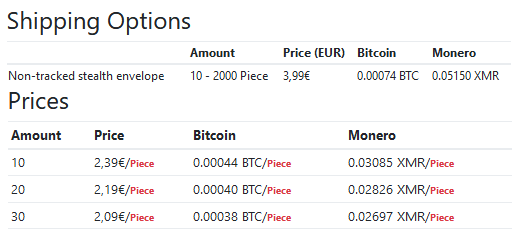
\includegraphics[trim={0 1.8cm 0 0},clip,width=0.71\textwidth]{Screenshot_360.png}
    \caption{Darknet market payment options.}
    \vspace{-1.5em}
    \label{pic:withoutresdrawable}
\end{center}
    \end{figure}


Although darknet markets may support Monero, a short inspection of top 10 markets revealed that only 5 of them list Monero as the general way to pay. Rest of them are not forcing the sellers to use Monero. This results at about 40\% availability of Monero payment option on these type of markets.


\chapter{Monero user research}
\label{cha:monerousersurvey}
The goal of this research is to gather information on end users behavior regarding Monero cryptocurrency with emphasis on key management and security practices. For this purpose, an online questionnaire was created. 

Specific survey design and research questions are based on Bitcoin security and privacy study, typical usage patterns of cryptocurrency users, online forums and Reddit communities centered around Monero as well as problematic areas regarding computer and data security in general \cite{krombholz2016other}.
\section{Research questions}
The survey was designed around seven question groups, some of them were shown only if the participant chose the appropriate answer.
\begin{itemize}\itemsep0em
\item G01 - Introductory information
\item G02 - Monero usage
\item G03 - Monero key and coin management
\item G04 - Monero and malicious things
\item G05 - Monero recovery
\item G06 - Special question set for miners
\item G07 - Demographics
\end{itemize}
Following this pattern, four research questions were set:
\begin{itemize}\itemsep0em
\item R1: What are Monero's main use cases? How do participants perceive Monero's features? 
\item R2: What are participant's ways of wallet access and storage?
\item R3: What security incidents have affected users? How did they deal with them?
\item R4: In case of recovery, how did they recover their keys?
\end{itemize}
\section{Participants and survey's background}
The significant characteristic of Monero is its anonymity, and this feature is not taken by community lightly. Due to this fact, the survey was not hosted on third party servers, but instead on dedicated VPS running Lime Survey self-hosted software with HTTPS interface using signed Letsencrypt certificates.

This means that data exchanged between participants and survey software stays only between these two parties, so Google or other big data company cannot analyze them. In order to allow extended anonymity features, Tor and proxy connections were allowed, but each participant had to solve the captcha before starting the survey.
\subsection{Methodology}
Data collection method was online only and was using the survey website software. Participants selection was based on opportunity sampling, links for the research were shared among dedicated Reddit Monero community, Facebook Monero groups as well as Cryptocurrency forums.

In order to reduce nonresponse rate, participants were asked only to fill out parts that were significant for them, e.g., Monero recovery part stayed hidden in the form if the user selected that he/she had never made any recovery of the seed or wallet keys in the previous part. 

The complete survey is attached in the chapter \ref{monero-user-study-pdf}.


\section{Results international, CZ}

\chapter{Monero usage and storage best practices}
Ease of use is one of the critical aspects of every cryptocurrency and although Monero can offer a wide range of anonymity features it has to be usable and user-friendly in order to be used by a substantial margin of people. Usability in Monero is a long-term topic that brings out active discussion \cite{monerolang2018}.

Following scenarios represent secure and easy to use instructions for a new Monero user.

\section{Generating the keys and accessing the wallet}
First challenge for Monero users is generating keypairs and accessing the wallet. This process varies from users platform of choice and used wallet software. As choice of client wallet software is fundamental for users Monero in terms of user experience and security standpoint, following sections are dedicated to avaiable wallet software.
\subsection{Windows and Linux platform}
The official client offers CLI and GUI wallet management and is available at \url{https://getmonero.org/downloads/}. Using the client users are able to generate the wallet keys. Created keys are after generation saved directly into the memory of the device unless specified otherwise. 
\begin{figure}[H]
\begin{center}
  %  \vspace{-0.8em}
 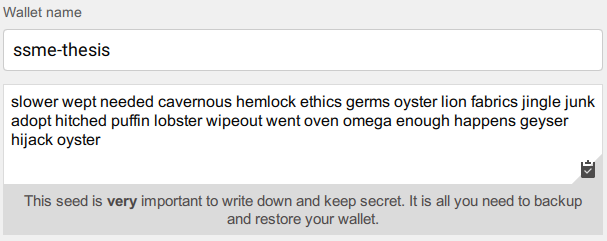
\includegraphics[trim={0 0 0 0},clip,width=0.85\textwidth]{Screenshot_4.png}
    \caption{GUI wallet generation}
  %  \vspace{-1.5em}
    \label{pic:guigenerator}
\end{center}
    \end{figure}

\begin{figure}[H]
\begin{center}
\begin{lstlisting}
.\monero-wallet-cli.exe
Monero 'Lithium Luna' (v0.12.3.0-release)
Logging to C:\...\monero-wallet-cli.log
Specify wallet file name (e.g., MyWallet). If the wallet 
doesn't exist, it will be created.
Wallet file name (or Ctrl-C to quit): ssme-thesis
No wallet found with that name. Confirm creation of new 
wallet named: ssme-thesis
(Y/Yes/N/No): Y
Generating new wallet...
\end{lstlisting}
\caption{CLI wallet generation}
    \label{pic:cligenerator}
\end{center}
    \end{figure}
Security of this task depends on the origin of the software, delivery chain trust, and the users' operating system. Monero CLI and GUI binaries can be edited, and the app itself does not call any internal checking to alert the user of the unauthorized change. 

   
Code injection was successfully tested on GUI binary of the official Monero wallet as seen in figure \ref{pic:codeinjectiongui}. Although SHA256 hash is provided on the website, the user is not specifically instructed to check the hashes of the downloaded software with tools like PowerShell using \texttt{Get-FileHash ./monero-wallet-gui.exe | Format-List} command \cite{pialphapialphagammaiotaacutealphanunualpharhoovarsigma2016study}. GPG-signed list of the hashes is avaiable on the website altough there are no instructions how to verify PGP signature itself.
\begin{figure}[H]
\begin{center}
\begin{lstlisting}
Algorithm : SHA256
Hash      : AF9324151909AC7B9BC6D622210EADFBAE5E66...
Path      : ./monero-wallet-gui-original.exe

Algorithm : SHA256
Hash      : DF4EC49E088284ECC78DBBD8B9CEFF00A78085...
Path      : ./monero-wallet-gui-injected.exe
\end{lstlisting}
\caption{Checksum change after code injeciton}
    \label{pic:codeinjectiongui}
\end{center}
    \end{figure}


%  Wallet key generation process is shown on examples in figures \ref{pic:cligenerator} and \ref{pic:guigenerator}. \\

There are also alternative approaches to key generation like an offline javascript based monero-wallet-generator that is available at \url{github.com/moneromooo-monero/monero-wallet-generator}.

\subsection{Hardware wallet}

Hardware way is considered to be in the development, but Monero compatibile devices like Ledger Nano S are already on the market. The way how keys are generated in hardware wallets varies on firmware included in each device. 

In general, the wallet is required to have Monero app installed from vendors app catalog. Keys are generated on the hardware device within the app itself and user can only export private view key from the device to view the balance in full CLI/GUI client.

This way, user has private spend key always on the device and client PC has only private view key. To sign a transaction, user has to confirm the transaction on the device itself meaning the hardware wallet will sign the transaction and then sends it to the Monero client. By this, in case of security breach on the host computer, there is no Monero to steal.

\subsection{Wallet software for mobile devices}

Monero has wallet software avaiable for Android as well as iOS platform. For both platforms community recommends users to use the open source ones, as their codebase is published on GitHub and everyone can inspect the code. Another common fact for the recommended solutions is that the keypairs for the wallet are stored exclusively on the users device and restore can be done without third party techsupport.

\textbf{Monerojuro} is an open source Android wallet application that is avaiable on Google Play as well as APK release at Github. By this, users can install the app from the Google Play directly, manually download the APK or compile it from sourcecode themselves. Wallet keys storage is based on the device only and the app encourages users to backup their seed.

\textbf{Monero Wallet} is an app released by Freewallet.org that provides Monero wallets for both Android and iOS. In terms of overall usability this app is easier for an average user as it does not present any cryptocurrency wallet terms as key, seed etc. User is instead instructed to create a Freewallet account which acts as a wallet. 

By this, user does not need to save the seed, wallet keys or make any backups as key management is completely on the side of service provider, Freewallet.org. This fact is often emphasised in Monero community as the user that does not control the keys, does not controll the wallet. Also source code is not publicly avaiable for community to review.

\textbf{Cake Wallet} represents open source  Monero wallet for iOS that provides wallet generation and local keypair storage with remote node connection and synchronization.

Guideline for secure wallet access is described in section \ref{sec:wallettypes}. 

\begin{figure}[H]
\begin{center}
\vspace{-0.75em}
 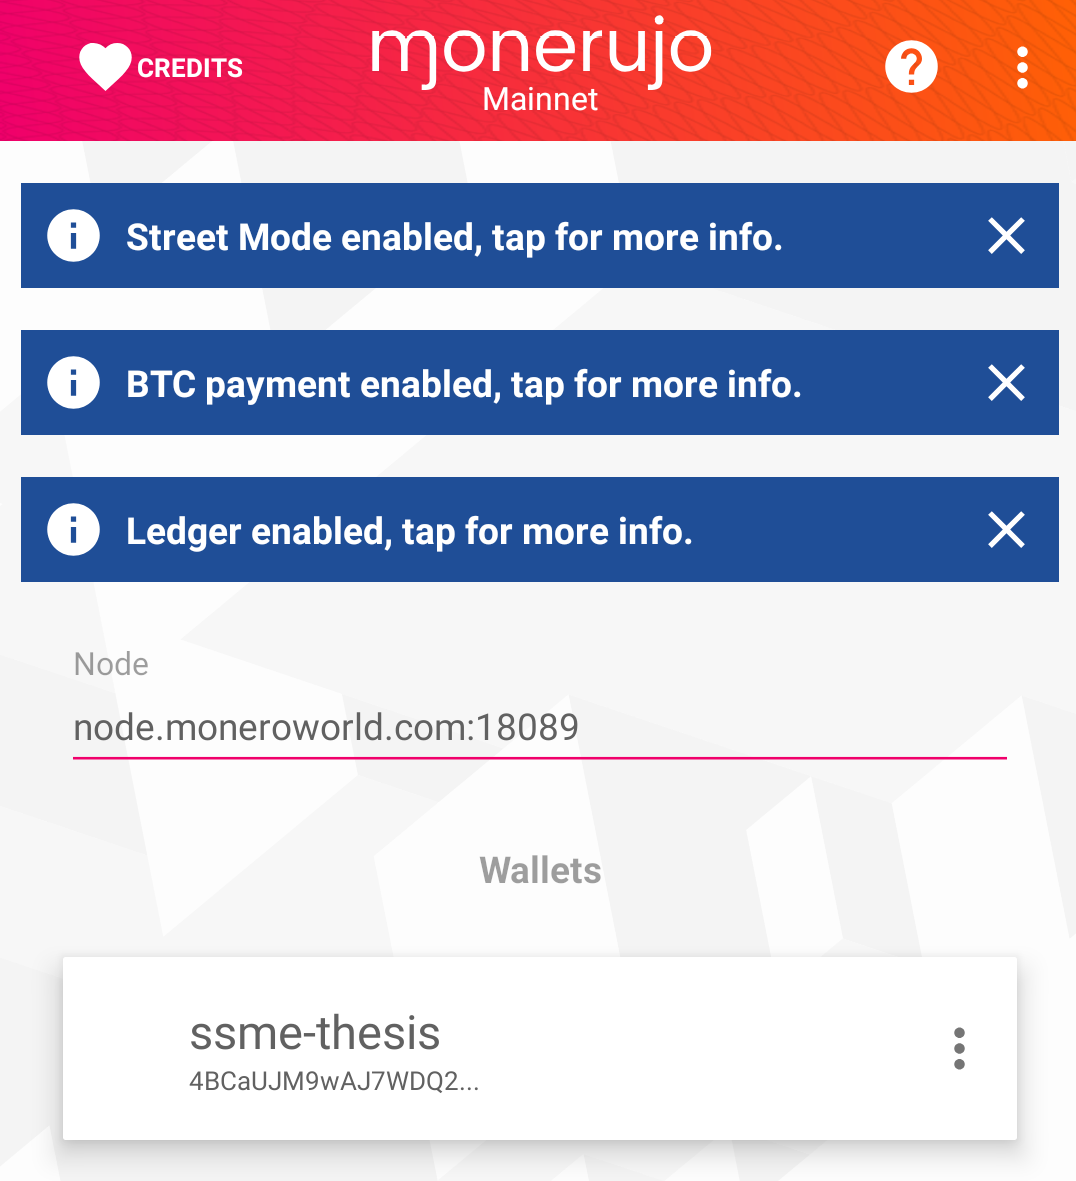
\includegraphics[trim={0 1.8cm 0 0},clip,width=0.55\textwidth]{Screenshot_1542566492.png}
    \caption{Monerujo for Android}
    \vspace{-1.5em}
    \label{pic:withoutresdrawable}
\end{center}
    \end{figure}
 \vspace{-0.9em}
\begin{figure}[H]
\centering\begin{tabular}{p{0.2\linewidth}p{0.15\linewidth}p{0.1\linewidth}p{0.4\linewidth}}
\textbf{Name}         & \textbf{Platform}      & \textbf{Source}        & \textbf{Wallet keys management} \\
Monerojuro    & Android       & Open Source   & Keypair is stored locally  User has complete control                       \\
Monero Wallet & Android  iOS & Closed Source & Keypair in cloud storage No control over keys \\
Cake Wallet   & iOS           & Open Source   & Keypair is stored locally  User has complete control                            
\end{tabular}
\captionof{table}{List of avaiable wallets for mobile platforms}
\label{table:monero-mobile}
\end{figure}


\section{Secure storage system}
Wallet keys are everything when it comes to cryptocurrency usage. Who has the keys, controlls the wallet and can view or transfer balance to another addresses. If user looses wallet keys, Monero wallet can still be recovered using mnemonic seed that should be saved on another storage medium. 

This section describes possible ways of backing-up wallet keys. Primary storage media security is compared in figure \ref{fig:walletstorage}.
\subsubsection{Data characteristics}
As described in section \ref{sec:wallets}, Monero wallet consists of encrypted \texttt{wallet.keys} file that contains private spend and view keys. Size of this file is less than a few kilobytes. 

Another type of data that is presented to the user is mnemonic seed. Seed can be used for recovery when wallet file is lost and consists of 25 words with the last one being used for checksum. 

In total, Monero wallet requires less than 8 kilobytes for key and seed storage. This results in minimal space requirements for backup storage media.

\subsection{Local storage}
\subsection{Network storage}
\subsection{Cloud storage}
\subsection{Backup rule}
\subsection{Testing the backups}

\subsubsection{}
\section{Secure usage pattern}
\section{Secure crypto portal}



\chapter{Obtaining Monero and running the network}
Monero mining is a process done by miners in order to verify transactions on the network and add them to the blockchain together in the form of a block. This results for them in a reward in the form of new coins that are emitted as a reward for block solving.

Network speed is mainly determined by the average time between individual blocks. %This results in transaction process that takes up to 130s (transaction request \textless 1s, network broadcast \textless 5s and transaction processing time as a time between submission and next mined block \textless 120 seconds). 
This results in transaction process that takes up to 130s (request =\textless 1s, broadcast =\textless 5s and max. time between blocks =\textless 120 seconds).  Transaction process is shown in figure \ref{pict:network-processing}.

\begin{figure}[H]
\center
\definecolor{ao(english)}{rgb}{0.0, 0.5, 0.0}
\definecolor{azure(colorwheel)}{rgb}{0.0, 0.5, 1.0}
\definecolor{darkorange}{rgb}{1.0, 0.55, 0.0}
\tikzstyle{decision} = [diamond, draw, fill=blue!20,
    text width=4.5em, text badly centered, node distance=2.5cm, inner sep=0pt]
\tikzstyle{userA} = [rectangle, draw, fill=ao(english)!20,
    text width=5em, text centered, rounded corners, minimum height=4em]
\tikzstyle{userB} = [rectangle, draw, fill=azure(colorwheel)!20,
    text width=5em, text centered, rounded corners, minimum height=4em]
\tikzstyle{userC} = [rectangle, draw, fill=darkorange!20,
    text width=5em, text centered, rounded corners, minimum height=4em]
\tikzstyle{lineuserA} = [draw, very thick, color=ao(english)!80, -latex']

\tikzstyle{lineuserB} = [draw, very thick, color=azure(colorwheel)!80, -latex']
\tikzstyle{lineuserC} = [draw, very thick, color=darkorange!80, -latex']
\tikzstyle{cloud} = [draw, ellipse,fill=red!20, node distance=2.5cm,
    minimum height=2em]

\begin{tikzpicture}[scale=2, node distance = 2cm, auto]
\shorthandoff{-}
    % Place nodes
    \node [userA,text width=5cm,minimum width=5cm] (userA1) {\parbox{5cm}{\centering Transaction request generated by the client \texttt{transfer ADDRESS AMOUNT}}};
    \node [userB, right of=userA1, node distance=6cm, text width=5cm,minimum width=5cm] (userB1)    {\parbox{5cm}{\centering Request broadcast to network nodes, shown \texttt{show_transfers pool} }};
    
    \node [below of=userA1,node distance=2.5cm,text width=5cm,minimum width=5cm, draw=none] (userA2){};
    \node [userB, below of=userB1, node distance=2.5cm,text width=5cm,minimum width=5cm] (userB2)    {\parbox{5cm}{\centering Transaction is added to the block waiting to be mined.}};
    
    \node [userC, below of=userA2,node distance=2.5cm,text width=5cm,minimum width=5cm] (userA3)  {\parbox{5cm}{\centering Miners are verifying transactions in the pending block.}}; %, in cli called multisig wallet password
    \node [userB, below of=userB2, node distance=2.5cm,text width=5cm,minimum width=5cm] (userB3)    {\parbox{5cm}{\centering Every 2 minutes new Monero block is mined and added to the blockchain.}}; %, in cli called multisig wallet password
    
    
    \node [userC, below of=userA3,node distance=2.5cm,text width=5cm,minimum width=5cm] (userA4) {\parbox{5cm}{\centering Miners are rewarded by block reward.}};
    \node [userB, below of=userB3, node distance=2.5cm,text width=5cm,minimum width=5cm] (userB4)    {\parbox{5cm}{\centering Receiving party's wallet becomes aware of the transaction.}};
        
   % \node [block, below of=init, node distance=2.5cm,text width=3cm,minimum width=3cm] (identify) {\parbox{3cm}{\centering Repackaging by reseller}};
%    \node [block, below of=identify, node distance=2.5cm,text width=3cm,minimum width=3cm] (evaluate) {\parbox{3cm}{\centering HW wallet bought by enduser}};
 %   \node [cloud, left of=identify, node distance=5cm] (update) {\parbox{3cm}{\centering Malicious scratchpad with seed  }};
  %  \node [block, below of=evaluate, node distance=2.5cm,text width=3cm,minimum width=3cm] (attacker) {\parbox{3cm}{\centering Attacker's database of wallets}};
    % Draw edges
    \path [lineuserC] (userA3) -- (userB3);
   % \path [lineuserA] (userA2) -- (userA4);
    \path [lineuserB] (userB1) -- (userB2);
    \path [lineuserB] (userB2) -- (userB3);
    \path [lineuserB] (userB3) -- (userB4);
    \path [lineuserB] (userB3) to[in=14,out=210,looseness=0] (userA4);
        \path [lineuserA] (userA1) to[in=-165,out=-15,looseness=0]  (userB1);
        \path [lineuserB] (userB1) to[in=15,out=165,looseness=0]   (userA1);
   % \path [line] (identify) -- (evaluate);
   %\path [line] (expert) -- (init);
  % \path [lineuserA] (userA2) |- (userB2);
\end{tikzpicture}
\caption{Monero network processing}
\label{pict:network-processing}
\end{figure}
\newpage
\section{Mining nodes}
As was mentioned in chapter 7, mining is the main reason for transaction processing in Monero network, and as the mining process has rewards for successfully solving the block, this encourages many different entities to mine.
Since Bitcoin started to gain popularity, mining has divided into five categories, that are described in the following sections:  
\iffalse
\begin{itemize}\topsep0em\parskip0em\parsep0em
\begin{minipage}{0.4\linewidth}
\item Mining in pools
\item Solo mining
\item Web mining
\end{minipage}
\begin{minipage}{0.4\linewidth}
\item Botnet mining
\item Cloud mining
\end{minipage}
\end{itemize}
\fi
\subsubsection{Mining in pools}
Very often, miners combine their computational resources into one of the pools on the network. Due to the higher total hash rate, there is a greater chance of solving the block thus gaining the reward of newly emitted coins. After solving each block, the reward is distributed equally to miners connected to the pool according to PPS (per-per-share) or PPLNS (per-per-last-number-of-shares) system \cite{tarasiewicz2015cryptocurrencies}.

As of 29.09.2018 total hash rate of the network was 577.72 Mh/s (100\%), in known pools 530.79 Mh/s (91.88\%) and unknown part of the network 46.93 Mh/s (8.12\%). Unknown part represents either pools that are not listed or solo miners on the network.

\begin{figure}[H]
\begin{center}
\begin{tikzpicture}[]
\tikzstyle{every node}=[font=\footnotesize]
\pie []
    {26.79/nanopool.org,
      19.17/minexmr.com,
      18.02/supportxmr.com,
      5.69/miningpoolhub.com,
      22.21/other pools,
      8.12/unknown}
      
      
     \end{tikzpicture}
     \end{center}
      \caption{Hash rate distribution in Monero network}
      \label{chart:range}

\end{figure}
\subsubsection{Solo mining}
Represents "all or nothing" approach when it comes to the rewarding system. As solo miner's hash rate has to compete against all other solo miners as well as big pools, the chance of solving the block is rather small \cite{cong2018decentralized}.

On the other side, when solo miner solves the block successfully, the whole block reward is assigned to the mining address. With high-end, multiple GPU setup, the miner can achieve about 3.2 Kh/s; this would mean chance about 0.46 \% of "winning" the block reward. 

\subsubsection{Web mining}
CryptoNight algorithm mining stands out above others in the way how cryptocurrency can be mined. For Monero there are JavaScript-based miners like CoinHive available, that results in individual websites embedding this script and mining using the visitor's resources. 

This can result up to 300 hashes per second for users with powerful CPUs and is a viable alternative to advertisements when visitors spend more than 10 minutes on the website \cite{papadopoulos2018truth}. Typical examples of this approach are warez websites offering free online movies and torrent trackers.
% Web mining: https://arxiv.org/pdf/1806.01994.pdf
\subsubsection{Botnet mining}
Using other peoples resources for mining, often also called crypto jacking (a more broad term for hidden cryptocurrency mining without users approval), have become increasingly popular in Monero. As the cryptocurrency provides anonymity features as well as a wide range of mining software that is available for every major platform.

In the current cloud era of computing, this represents vast problems for both service providers and their customers. Providers experience increased power consumption, cooling requirements, customers, on the other hand, are required to pay more for consumed system resources \cite{tahir2017mining}.

\subsubsection{Cloud mining}
\definecolor{ao(english)}{rgb}{0.0, 0.5, 0.0}
\definecolor{azure(colorwheel)}{rgb}{0.0, 0.5, 1.0}
\definecolor{darkorange}{rgb}{1.0, 0.55, 0.0}
Represents managed services by specialists that offer mining power using cloud service providers. Due to managed service providers (MSP) markup, this way of mining is not as profitable and not recommended among Monero community in general. \\Arrows indicate flow of the resources:\\ \textcolor{ao(english)} {Payment for service}; \textcolor{azure(colorwheel)}{Payment for compute time}; \textcolor{darkorange}{Delivered hashrate}

\begin{figure}[H]
\center
\tikzstyle{decision} = [diamond, draw, fill=blue!20,
    text width=4.5em, text badly centered, node distance=2.5cm, inner sep=0pt]
\tikzstyle{userA} = [rectangle, draw, fill=ao(english)!20,
    text width=5em, text centered, rounded corners, minimum height=4em]
\tikzstyle{userB} = [rectangle, draw, fill=azure(colorwheel)!20,
    text width=5em, text centered, rounded corners, minimum height=4em]
\tikzstyle{userC} = [rectangle, draw, fill=darkorange!20,
    text width=5em, text centered, rounded corners, minimum height=4em]
\tikzstyle{lineuserA} = [draw, very thick, color=ao(english)!80, -latex']

\tikzstyle{lineuserB} = [draw, very thick, color=azure(colorwheel)!80, -latex']
\tikzstyle{lineuserC} = [draw, very thick, color=darkorange!80, -latex']
\tikzstyle{cloud} = [draw, ellipse,fill=red!20, node distance=2.5cm,
    minimum height=2em]

\begin{tikzpicture}[scale=2, node distance = 0.4cm, auto]
\shorthandoff{-}
    % Place nodes
    \node [userA,text width=2cm,minimum width=2cm] (userA1) {\parbox{2cm}{\centering Hashrate buyer}};
    \node [userB, right of=userA1, node distance=4cm, text width=2cm,minimum width=2cm] (userB1)    {\parbox{2cm}{\centering MSP }};
    \node [userC, right of=userB1, node distance=4cm, text width=2cm,minimum width=2cm] (userC1)    {\parbox{2cm}{\centering Datacentre }};
        
   % \node [block, below of=init, node distance=2.5cm,text width=3cm,minimum width=3cm] (identify) {\parbox{3cm}{\centering Repackaging by reseller}};
%    \node [block, below of=identify, node distance=2.5cm,text width=3cm,minimum width=3cm] (evaluate) {\parbox{3cm}{\centering HW wallet bought by enduser}};
 %   \node [cloud, left of=identify, node distance=5cm] (update) {\parbox{3cm}{\centering Malicious scratchpad with seed  }};
  %  \node [block, below of=evaluate, node distance=2.5cm,text width=3cm,minimum width=3cm] (attacker) {\parbox{3cm}{\centering Attacker's database of wallets}};
    % Draw edges
        \path [lineuserA] (userA1) -- (userB1);
        %\path [lineuserB] (userB1) to[in=15,out=165,looseness=0]   (userA1);
        \path [lineuserB] (userB1) --  (userC1);
        \path [lineuserC] (userC1) to[in=35,out=145,looseness=1]   (userA1);
   % \path [line] (identify) -- (evaluate);
   %\path [line] (expert) -- (init);
  % \path [lineuserA] (userA2) |- (userB2);
\end{tikzpicture}
\caption{Monero network processing}
\label{pict:network-processing}
\end{figure}

\section{Mining software}
\subsubsection{Official}
Can be obtained at the official web of the Monero cryptocurrency project at https://getmonero.org/downloads/ . This is an official wallet software that includes solo mining client and cannot be used for pool mining.

\subsubsection{Community-driven}
Is a category that incorporates opensource mining software projects that have source code published on the Github. Mostly used are:

\begin{itemize}\itemsep0em
\item XMR Stak 
\begin{itemize}\itemsep0em \item Consolidates CPU, AMD and Nvidia GPU mining under one multiplatform application with integrated webserver and autoconfiguration capability. \item Url: \url{https://github.com/fireice-uk/xmr-stak} \end{itemize}
\setlength\itemsep{1em}
\item XMRig 
\setlength\itemsep{0em}
\begin{itemize}\itemsep0em \item Three separately released miners with autoconfiguration GPU and CPU capability. \item AMD: \url{https://github.com/xmrig/xmrig-amd} 
 \item Nvidia: \url{https://github.com/xmrig/xmrig-nvidia} \item CPU: \url{https://github.com/xmrig/xmrig} \end{itemize}
\item CCminer - Nvidia CUDA miner
\begin{itemize}\itemsep0em \item Url: \url{https://github.com/tpruvot/ccminer/} \end{itemize}
\end{itemize}

\begin{figure}[H]
\begin{center}

    \vspace{-0.8em}
 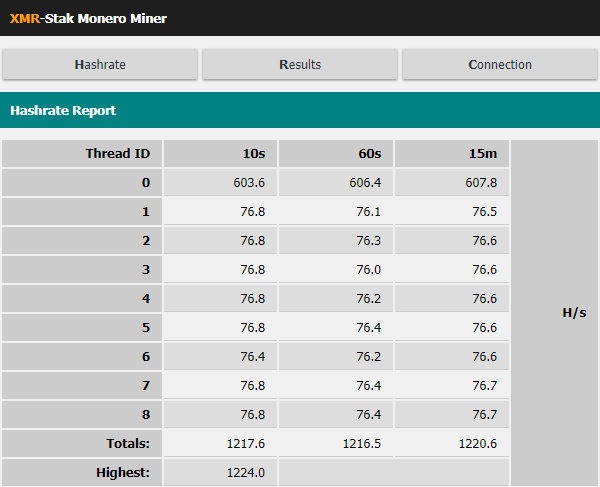
\includegraphics[trim={0 0 0 0},clip,width=0.85\textwidth]{Screenshot_9.png}
    \caption{XMR-Stak web interface}
    \vspace{-1.5em}
    \label{pic:withoutresdrawable}
\end{center}
    \end{figure}
    
\subsubsection{Proprietary}
Having closed source code that community cant inspect, mining software of this category has less reputation compared to the community-driven. This is caused mainly by the fact that the exact produced hash rate and client reported hash rate differed in the past at least regarding the MinerGate miner available at \url{https://minergate.com/downloads/gui} .
\iffalse
\section{XMR obtaining comparison}
\begin{figure}[H]
\center
\begin{tabular}{p{0.2\linewidth}p{0.16\linewidth}p{0.16\linewidth}p{0.16\linewidth}p{0.16\linewidth}p{0.16\linewidth}}
\textbf{Mining type} & \textbf{Security} & \textbf{Depenence} & \textbf{Payout} & \textbf{Avaiability} & \textbf{Profitability} \\
Pool mining          &                   &                    &                 &                      &                        \\
Solo mining          &                   &                    &                 &                      &                        \\
Web mining           &                   &                    &                 &                      &                        \\
Botnet mining        &                   &                    &                 &                      &                        \\
Cloud mining         &                   &                    &                 &                      &                       
\end{tabular}
\caption{Monero network processing}
\label{pict:network-processing}
\end{figure}
\fi
\chapter{Monero miners research}
%tento výzkum jsem nenašel, takže říct, že tam nic dalšího není napsat to tam
%zobrazování voleb pro multiple choice randomizovat
% total hardware dát pryč a místo toho jen hashrate OK
%obtain software > official github OK
%2x mám incident OK
%pooly podle abecedy OK
%vypustit verzi windows OK
%other u linux os OK
%mining os dodat OK
% škola > dodá Vlasta info
% místo interested in modern technologies >> eearly adopter OK
% privacy aspect vygooglit části
The goal of this research is to gather information on people who run mining cryptocurrency software and map their behavior regarding system administration with the emphasis on security practices. For this purpose, an online questionnaire was created. 

To the best of my knowledge, this is the first work that studies cryptocurrency miners. Specific research questions are based on cryptocurrency mining setup patterns, used software and problematic areas regarding computer and data security in general. 

\section{Research questions}
The survey was designed around seven question groups, some of them were shown only if the participant chose the appropriate answer.
\begin{itemize}\itemsep0em
\item G01 - Introductory information
\item G02 - Mining setup
\item G03 - Mining software
\item G04 - Pool choice
\item G05 - Windows platform
\item G06 - Linux platform
\item G07 - Demographics
\end{itemize}
Following this pattern, five research questions were set:
\begin{itemize}\itemsep0em
\item R1: Who are Monero miners in general? What are their typical mining setups? 
\item R2: Which types of software do participants use as operating systems, management, and mining tools?
\item R3: What security and update policies miners follow? 
\item R4: Do miners suffer from security incidents like compromised mining operation? How do they deal with them?
\item R5: What are the factors that affect pool choice?
\end{itemize}
\section{Participants and survey's background}
As mentioned in chapter \ref{cha:monerouserresearch}, the survey was not hosted on third party servers, but instead on dedicated VPS running Lime Survey self-hosted software with HTTPS interface using signed Letsencrypt certificates.

This means that data exchanged between participants and survey software stays only between these two parties, so Google or other big data company cannot analyze them. In order to allow extended anonymity features, Tor and proxy connections were allowed, but each participant had to solve the captcha before starting the survey.
\subsection{Methodology}
Data collection method was online only and was using the survey website software. Participants selection was based on opportunity sampling, links for the research were shared among dedicated Reddit Monero community, Facebook Mining groups as well as Cryptocurrency forums. This form was distributed together with the Monero User Research survey in mentioned mining communities.

In order to reduce nonresponse rate, participants were asked only to fill out parts that were significant for them, e.g., Windows OS part stayed hidden in the form if the user selected that he/she used Linux OS only. 

Complete survey is attached in chapter \ref{monero-miner-study-pdf}.
\section{Results international, CZ}



\chapter{Monero pool operators research}
The goal of this research is to gather information about people who run mining pools and are indirectly responsible for Monero transactions processing. The research aims to map mining pool administration consisting of coin management, attacks mitigation, and disaster recovery scenarios. For this purpose, an online questionnaire was created. 

To the best of my knowledge, this is the first work that studies cryptocurrency pool operators. Specific research questions are based on available pool software, infrastructure services, hosting software and problematic areas regarding computer and data security in general.

\section{Research questions}
%antiDDOS!!!!! OK
%co znamena zaloha poolu rozepsat OK

The survey was designed around five question groups, some of them were shown only if the participant chose the appropriate answer.
\begin{itemize}\itemsep0em
\item G01 - Introductory information
\item G02 - Coin management
\item G03 - Defending against attackers
\item G04 - Backups and disaster recovery
\item G05 - Demographics
\end{itemize}
Following this pattern, four research questions were set:
\begin{itemize}\itemsep0em
\item R1: What technical infrastructure background is typical for pool operations?
\item R2: How do pool operators manage pool wallet and coins in general?
\item R3: Do pool operators use any attack mitigation services?
\item R4: What are backup solutions do pool operators use?
\end{itemize}
\section{Participants and survey's background}
As mentioned in chapter \ref{cha:monerousersurvey}, the survey was not hosted on third party servers, but instead on dedicated VPS running Lime Survey self-hosted software with HTTPS interface using signed Letsencrypt certificates.

This means that data exchanged between participants and survey software stays only between these two parties, so Google or other big data company cannot analyze them. In order to allow extended anonymity features, Tor and proxy connections were allowed, but each participant had to solve the captcha before starting the survey.
\subsection{Methodology}
Data collection method was online only and was using the survey website software. Participants selection was based on systematic sampling as links for the research were sent to the pool operators only.

Complete survey is attached in chapter \ref{monero-pool-study-pdf}.
\section{Results international, CZ}

 
\chapter{Mining malware}
\section{Prevention, detection and recovery}
\subsection{Systems administrators perspective}
%kitty https://www.incapsula.com/blog/crypto-me0wing-attacks-kitty-cashes-in-on-monero.html
\subsection{Regular users}


\chapter{Designing secure mining environment}
\section{Linux-based solution}
Ansible, Centos 7
\section{Windows-based solution}
Windows 10 ISO unattended install, Powershell scripts, XMR-stak

\chapter{Plan}

\begin{figure}[H]
\center
\begin{tabular}{ll}
Month     & Task                                              \\
1.7.2018  & Monero cryptocurrency; Monero Usage              \\
1.8.2018  & Research design  \\
1.9.2018  & Data collection; Monero mining and running the network \\
1.10.2018 & Data summary                                   \\
1.11.2018 & Best practices for usage and storage                \\
1.12.2018 & Mining malware; Secure mining system design     \\
1.1.2019  & Cryptocore.cz web            \\
1.2.2019  & Spare time                                           \\
1.3.2019  & Month for completion                                 \\
1.4.2019  & Final version + print                            
\end{tabular}
\caption{Diploma thesis plan}
\label{ssme-thesis-plan}
\end{figure}



\printbibliography[heading=bibintoc]

\appendix
\includepdf[pages=1,pagecommand=\chapter{Monero User Survey},scale=0.7]{monerousersurvey.pdf}
\label{monero-user-study-pdf}
\includepdf[pages={2,3,4,5,6,7,8,9},scale=0.7, pagecommand={}]{monerousersurvey.pdf}
\includepdf[pages=1,pagecommand=\chapter{Monero Miners Survey},scale=0.7]{monerominersurvey.pdf}
\label{monero-miners-study-pdf}
\includepdf[pages={2,3,4,5,6,7,8,9,10},scale=0.7, pagecommand={}]{monerominersurvey.pdf}
\includepdf[pages=1,pagecommand=\chapter{Monero User Survey},scale=0.7]{moneropoolsurvey.pdf}
\label{monero-pool-study-pdf}
\includepdf[pages={2,3,4,5},scale=0.7, pagecommand={}]{moneropoolsurvey.pdf}
 %% Start the appendices.
%\chapter{Zdroje k tabulce 2.2}
%dash https://bitcointalk.org/index.php?topic=1562109.0
%dash https://docs.dash.org/en/latest/introduction/information.html
%pivx https://github.com/PIVX-Project/PIVX
%pivx https://www.reddit.com/r/pivx/comments/7gjjyw/what_are_the_benefits_of_multisig_addresses/
%zcoin https://github.com/zcoinofficial/zcoin/wiki/Information-for-exchanges
%zcoin https://zcoin.io/zcoins-privacy-technology-compares-competition/
\end{document}
